\documentclass[a4paper,12pt]{article}

\usepackage{amsmath,amssymb,amsthm,tikz}
\usetikzlibrary{calc,arrows.meta}
\usepackage[margin=20mm]{geometry}

\setlength{\parindent}{0pt}
\setlength{\columnsep}{1cm}

\begin{document}

%\twocolumn

\thispagestyle{empty}

\begin{center}
{\Large Assignment 6}\\
{\Large 2020-10-28,}\\
{\em 12 minutes} 
\end{center}

\noindent


\vspace{10pt}
{\bf Question 1 (Removing from Maximum Heap}

\begin{figure}[!htb]
\center{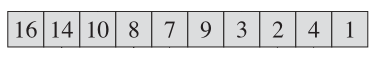
\includegraphics[width=3in]{assignment06-heaps/heap-problem.png}}
\caption{\label{fig:unsorted-heap} Array for a Max-Heap}
\end{figure}

The image shows array used to store Maximum Heap 
(a data structure allowing inserts and removal of the maximum element). 
The array starts with the $0$th element 
(and any parent node in such tree should always be at least as big as 
any of its children). 

\vspace{5pt}
{\bf (A)} Draw the initial heap based on this array. 
Heap should be drawn as a complete 
binary tree.

\vspace{5pt}
{\bf (B)} Run the command $\text{\sc DeleteMax}(H)$
on this initial heap. Draw the resulting binary tree (after the heap 
invariant is restored \textendash{} any parent node is
at least as big as its children). 
Draw the binary tree image you get.

\vspace{5pt}
{\bf (C)} On the tree that you got in the previous step {\bf (B)}
run the command $\text{\sc Insert}(H,x)$, 
where $x = a+b+c$ is the sum of the last three digits of your student ID. 
Draw the binary tree image you get.

\vspace{5pt}
{\bf (D)} Show the array for the binary tree you got in the previous step {\bf (C)}
(i.e.\ right after the\\ $\text{\sc DeleteMax}(H)$ and $\text{\sc Insert}(H,x)$ commands 
have been executed). 



\end{document}



